% Q17 -- Parity 1-bit CMOS cell STICK diagram (simplified, colour-coded).
% p-diffusion (yellow) above the dashed demarcation line, n-diffusion (green) below;
% red poly gates cross both; blue metal/rails; black contacts.
\documentclass[border=10pt]{standalone}
\usepackage{tikz}
\begin{document}
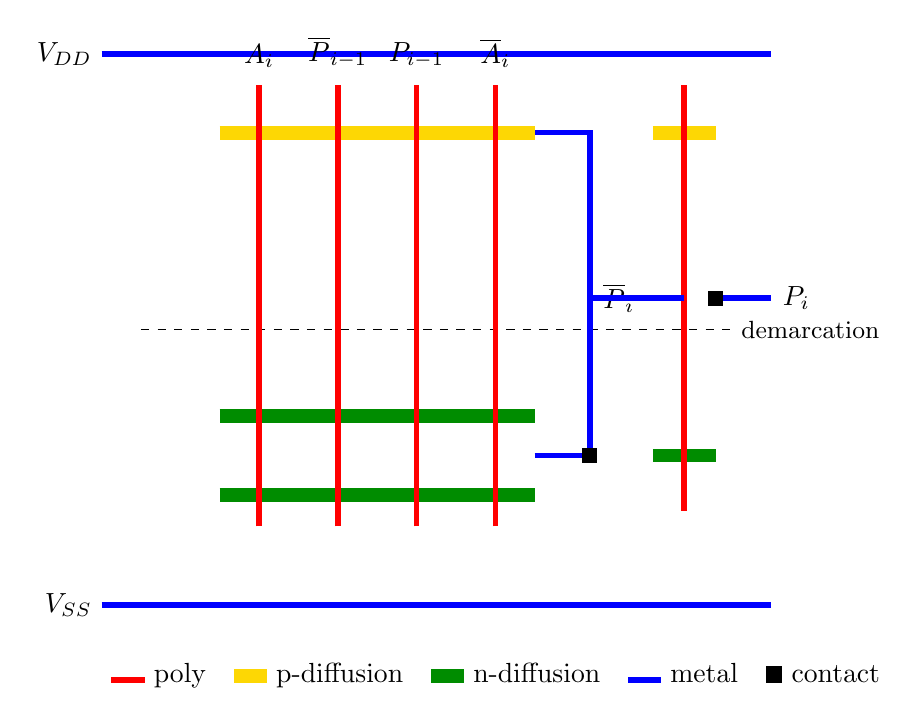
\begin{tikzpicture}[
  poly/.style={red, line width=2pt},
  ndiff/.style={green!55!black, line width=5pt},
  pdiff/.style={yellow!75!orange, line width=5pt},
  metal/.style={blue, line width=2pt},
  cont/.style={fill=black, draw=black, minimum size=5pt, inner sep=0pt}]
% rails
\draw[metal] (0,7) -- (8.5,7); \node[left] at (0,7){$V_{DD}$};
\draw[metal] (0,0) -- (8.5,0); \node[left] at (0,0){$V_{SS}$};
% demarcation line
\draw[dashed] (0.5,3.5) -- (8.0,3.5); \node[right] at (8.0,3.5){\small demarcation};
% p-diffusion (top) -- p-block
\draw[pdiff] (1.5,6) -- (5.5,6);
% n-diffusion (bottom) -- two branches
\draw[ndiff] (1.5,1.4) -- (5.5,1.4);
\draw[ndiff] (1.5,2.4) -- (5.5,2.4);
% poly gates crossing both blocks
\foreach \c/\lbl in {2/$A_i$,3/$\overline{P}_{i-1}$,4/$P_{i-1}$,5/$\overline{A}_i$}{
  \draw[poly] (\c,1.0) -- (\c,6.6);
  \node[above] at (\c,6.7) {\lbl};
}
% metal node Pbar_i tying p-block and n-block outputs
\draw[metal] (5.5,1.9) -- (6.2,1.9) -- (6.2,6) -- (5.5,6);
\node[right] at (6.25,3.9){$\overline{P}_i$};
% inverter stage -> P_i
\draw[pdiff] (7.0,6) -- (7.8,6);
\draw[ndiff] (7.0,1.9) -- (7.8,1.9);
\draw[poly] (7.4,1.2) -- (7.4,6.6);
\draw[metal] (6.2,3.9) -- (7.4,3.9);
\draw[metal] (7.8,3.9) -- (8.5,3.9) node[right,black]{$P_i$};
\node[cont] at (6.2,1.9){}; \node[cont] at (7.8,3.9){};
% legend
\node[anchor=west, align=left] at (0,-0.9)
 {\textcolor{red}{$\rule{12pt}{2pt}$} poly\quad
  \textcolor{yellow!75!orange}{$\rule{12pt}{5pt}$} p-diffusion\quad
  \textcolor{green!55!black}{$\rule{12pt}{5pt}$} n-diffusion\quad
  \textcolor{blue}{$\rule{12pt}{2pt}$} metal\quad
  \rule{6pt}{6pt}~contact};
\end{tikzpicture}
\end{document}
